\chapter{Z Tanım Bölgesinde Durum Uzayı}

Yay-kütle-damper sisteminin dinamikleri $x(t)$ yer değiştirme olmak üzere
\begin{equation}
    m\ddot{x}(t)+b\dot{x}(t)+kx(t)=u(t)
\end{equation}
ile verilmiştir. Verilen ikinci dereceden diferansiyel denklemi iki adet birinci dereceden diferansiyel denkleme çevirmek mümkündür. Bunun için $x_1(t)\triangleq x(t)$ tanımlanır ve
\begin{equation}
\begin{split}
    \dot{x}_1(t)&=\dot{x}(t)\triangleq x_2(t)\\
    \dot{x}_2(t)&=\ddot{x}(t)
\end{split}
\end{equation}
tanımlanır. Bu durumda,
\begin{equation}
    \begin{split}
        m\ddot{x}(t)+b\dot{x}(t)+kx(t)=u(t)\\
        m\dot{x}_2(t)+bx_2(t)+kx_1(t)=u(t)\\
        m\dot{x}_2(t)=-bx_2(t)-kx_1(t)+u(t)\\
        \dot{x}_2(t)=-\frac{b}{m}x_2(t)-\frac{k}{m}x_1(t)+\frac{1}{m}u(t)
    \end{split}
\end{equation}
elde edilir. Diferansiyel denklem takımı
\begin{equation}
    \begin{split}
        \dot{x}_1(t)&=x_2(t)\\
        \dot{x}_2(t)&=-\frac{b}{m}x_2(t)-\frac{k}{m}x_1(t)+\frac{1}{m}u(t)
    \end{split}
\end{equation}
ve hatta 
\begin{equation}
    \begin{bmatrix}
        \dot{x}_1(t)\\
        \dot{x}_2(t)
    \end{bmatrix}=
    \begin{bmatrix}
        0& 1\\
        -\frac{k}{m}& -\frac{b}{m}
    \end{bmatrix}\begin{bmatrix}
        x_1(t)\\
        x_2(t)
    \end{bmatrix}+\begin{bmatrix}
        0\\
        \frac{1}{m}
    \end{bmatrix}u(t)
\end{equation}
elde edilir. Sistem için parametreler $m=1$, $b=0.5$ ve $k=1$ olmak üzere durum uzayı modeli
\begin{equation}
\begin{split}
    \begin{bmatrix}
        \dot{x}_1(t)\\
        \dot{x}_2(t)
    \end{bmatrix}&=
    \begin{bmatrix}
        0& 1\\
        -1& -0.5
    \end{bmatrix}\begin{bmatrix}
        x_1(t)\\
        x_2(t)
    \end{bmatrix}+\begin{bmatrix}
        0\\
        1
    \end{bmatrix}u(t)\\
    y(t)&=\begin{bmatrix}
        1&0 
    \end{bmatrix}\begin{bmatrix}
        x_1(t)\\
        x_2(t)
    \end{bmatrix}
\end{split}
\end{equation}
olarak elde edilir. \verb|Simulink| modeli Şekil~\ref{fig:model1} ile verilmiştir.
\begin{figure}[!htb]
    \centering
    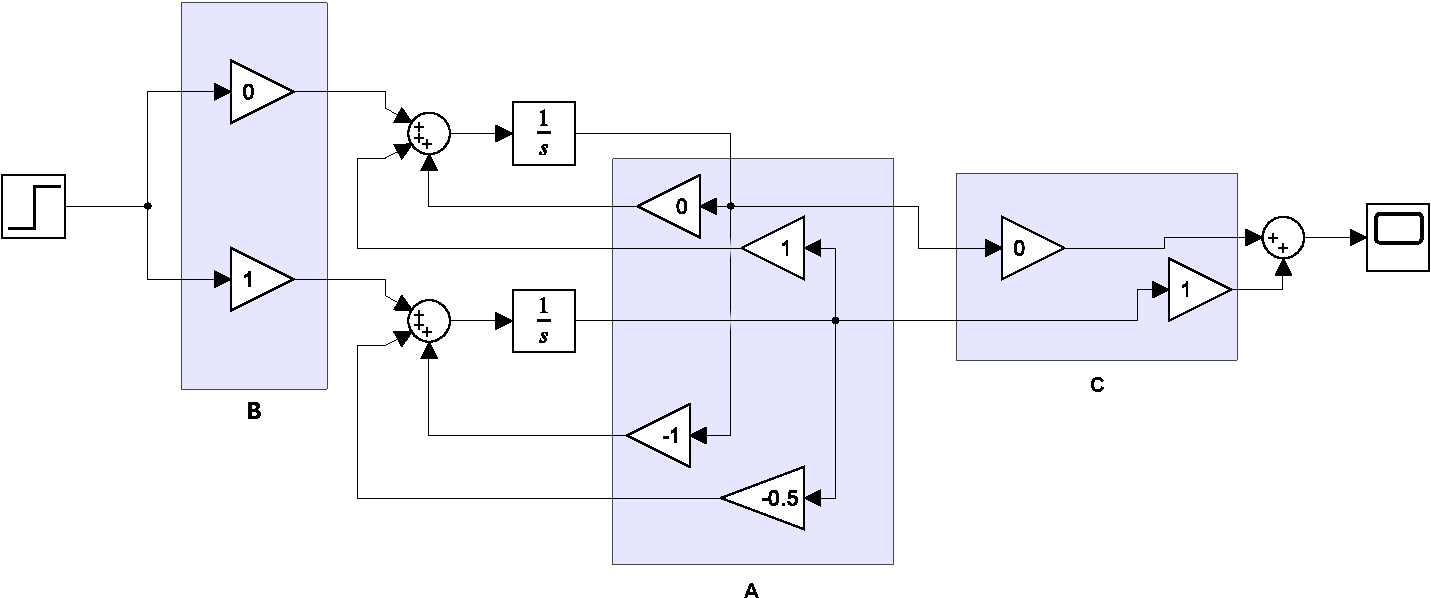
\includegraphics[width=\textwidth]{img/model1}
    \caption{Yay-kütle-damper sistemine ait durum uzay modeli}
    \label{fig:model1}
\end{figure}

Ayrık durum uzayı ZOH yöntemi ile türevin yorumuna dayanmaktadır ve 
\begin{equation}
    \frac{dx}{dt}=\frac{\Delta x}{\Delta t}=\frac{x(kT)-x((k-1)T)}{T}
\end{equation}
ile durum uzayı
\begin{equation}
    \begin{split}
        \frac{1}{T}\begin{bmatrix}
            x_1(kT)-x_1((k-1)T)\\
            x_2(kT)-x_2((k-1)T)
        \end{bmatrix}&=
        \begin{bmatrix}
            0& 1\\
            -1& -0.5
        \end{bmatrix}\begin{bmatrix}
            x_1((k-1)T)\\
            x_2((k-1)T)
        \end{bmatrix}+\begin{bmatrix}
            0\\
            1
        \end{bmatrix}u((k-1)T)\\
        y((k-1)T)&=\begin{bmatrix}
            1&0 
        \end{bmatrix}\begin{bmatrix}
            x_1((k-1)T)\\
            x_2((k-1)T)
        \end{bmatrix}
    \end{split}
\end{equation}
olarak elde edilmektedir. Matematiksel işlemler sonucu
\begin{equation}
    \begin{split}
        \begin{bmatrix}
            x_1(kT)\\
            x_2(kT)
        \end{bmatrix}&=
        \begin{bmatrix}
            1&0\\
            0&1
        \end{bmatrix}
        \begin{bmatrix}
            x_1((k-1)T)\\
            x_2((k-1)T)
        \end{bmatrix}+
        T\begin{bmatrix}
            0& 1\\
            -1& -0.5
        \end{bmatrix}\begin{bmatrix}
            x_1((k-1)T)\\
            x_2((k-1)T)
        \end{bmatrix}+\begin{bmatrix}
            0\\
            T
        \end{bmatrix}u((k-1)T)\\
        y((k-1)T)&=\begin{bmatrix}
            1&0 
        \end{bmatrix}\begin{bmatrix}
            x_1((k-1)T)\\
            x_2((k-1)T)
        \end{bmatrix}
    \end{split}
    \end{equation}
    ve sonuç olarak
        \begin{equation}
            \begin{split}
        \begin{bmatrix}
            x_1(kT)\\
            x_2(kT)
        \end{bmatrix}&=
        \begin{bmatrix}
            1& T\\
            -T& 1-0.5T
        \end{bmatrix}\begin{bmatrix}
            x_1((k-1)T)\\
            x_2((k-1)T)
        \end{bmatrix}+\begin{bmatrix}
            0\\
            T
        \end{bmatrix}u((k-1)T)\\
        y((k-1)T)&=\begin{bmatrix}
            1&0 
        \end{bmatrix}\begin{bmatrix}
            x_1((k-1)T)\\
            x_2((k-1)T)
        \end{bmatrix}\\
    \end{split}
\end{equation}
elde edilir. Örnekleme zamanı $T=0.1$ olmak üzere durum uzayı modeli
\begin{equation}
    \begin{split}
\begin{bmatrix}
    x_1[k]\\
    x_2[k]
\end{bmatrix}&=
\begin{bmatrix}
    1& 0.1\\
    -0.1& 0.95
\end{bmatrix}\begin{bmatrix}
    x_1[k-1]\\
    x_2[k-1]
\end{bmatrix}+\begin{bmatrix}
    0\\
    0.1
\end{bmatrix}u[k-1]\\
y[k-1]&=\begin{bmatrix}
    1&0 
\end{bmatrix}\begin{bmatrix}
    x_1[k-1]\\
    x_2[k-1]
\end{bmatrix}\\
\end{split}
\end{equation}
şeklindedir. Durum uzayı modeli denklemleri
\begin{equation}
    \begin{split}
    x_1[k]&=x_1[k-1]+0.1x_2[k-1]\\
    x_2[k]&=-0.1x_1[k-1]+0.95x_2[k-1]+0.1u[k-1]\\
    y[k-1]&=x_1[k-1]
\end{split}
\end{equation}
şeklindedir. Girişine $sin(4t)$ uygulandığında elde edilen yanıt Şekil~\ref{fig:lec11_plot1} ile verilmiştir.
\begin{figure}[!htb]
    \centering
    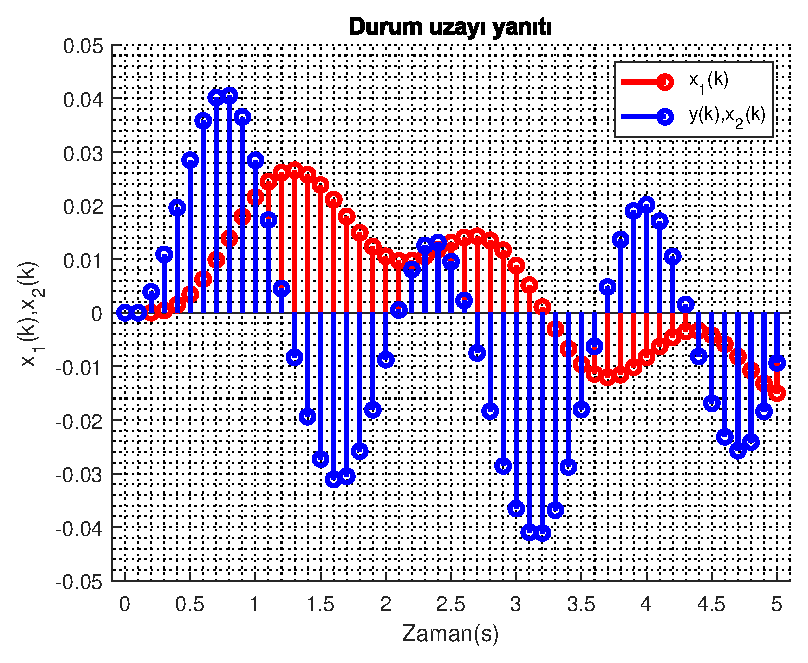
\includegraphics[width=0.75\textwidth]{img/lec11_plot1}
    \caption{Yay-kütle-damper sistemine ait durum uzay modeli yanıtı}
    \label{fig:lec11_plot1}
\end{figure}

\verb|Simulink| modeli Şekil~\ref{fig:model2} ile verilmiştir.
\begin{figure}[!htb]
    \centering
    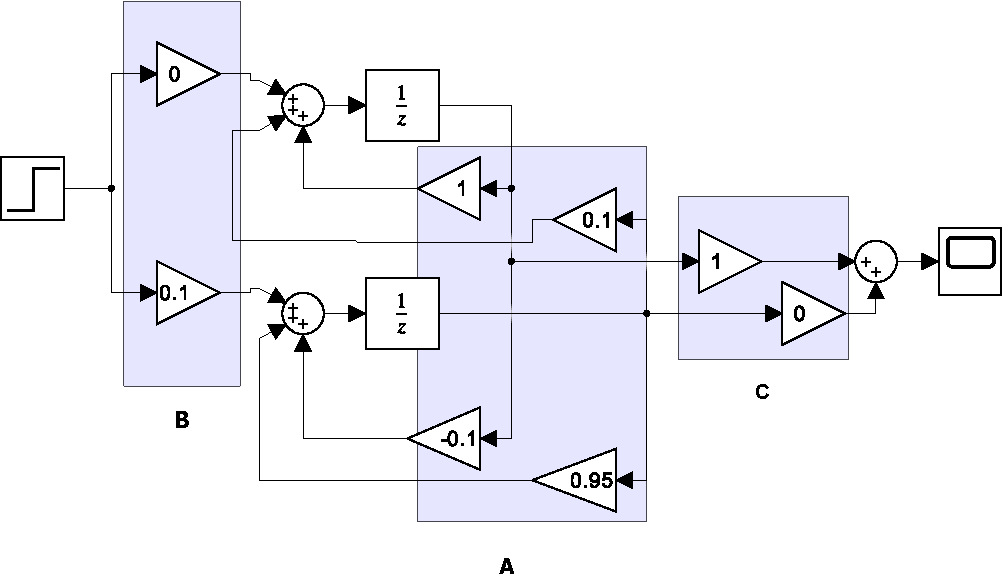
\includegraphics[width=\textwidth]{img/model2}
    \caption{Yay-kütle-damper sistemine ait ayrık durum uzay modeli}
    \label{fig:model2}
\end{figure}
